Til visualisering af data er der anvendt html/CSS/Javascript, disse data kommer fra vores \texttt{Models} som bliver manipuleret af \texttt{Controller}, som brugeren anvender til at ses, tilføje, slette og ændre data, som illustreret på figur \ref{fig:Diagram_WebView}.
\newline
\newline
Under view i Web Api er der tilføjet 3 view, \texttt{Index}, \texttt{Settings}, og \texttt{Statistic}, dette er 3 html sider, hvor der er anvendt bootstrap til style, form elementer, panels og knapper. Her er der også anvendt knockout data binding attributter, disse binder knockout view models til html elementer, som bliver specificeret i et data-binding udtryk. 
\newline
\newline
De forskellige view-models er defineret i en view model javascript fil, hvor de så bliver gemt som knockout Observable Arrays eller observables, med de værdier der står i databasen. 
\newline
\newline
\begin{figure}[H]
	\centering
	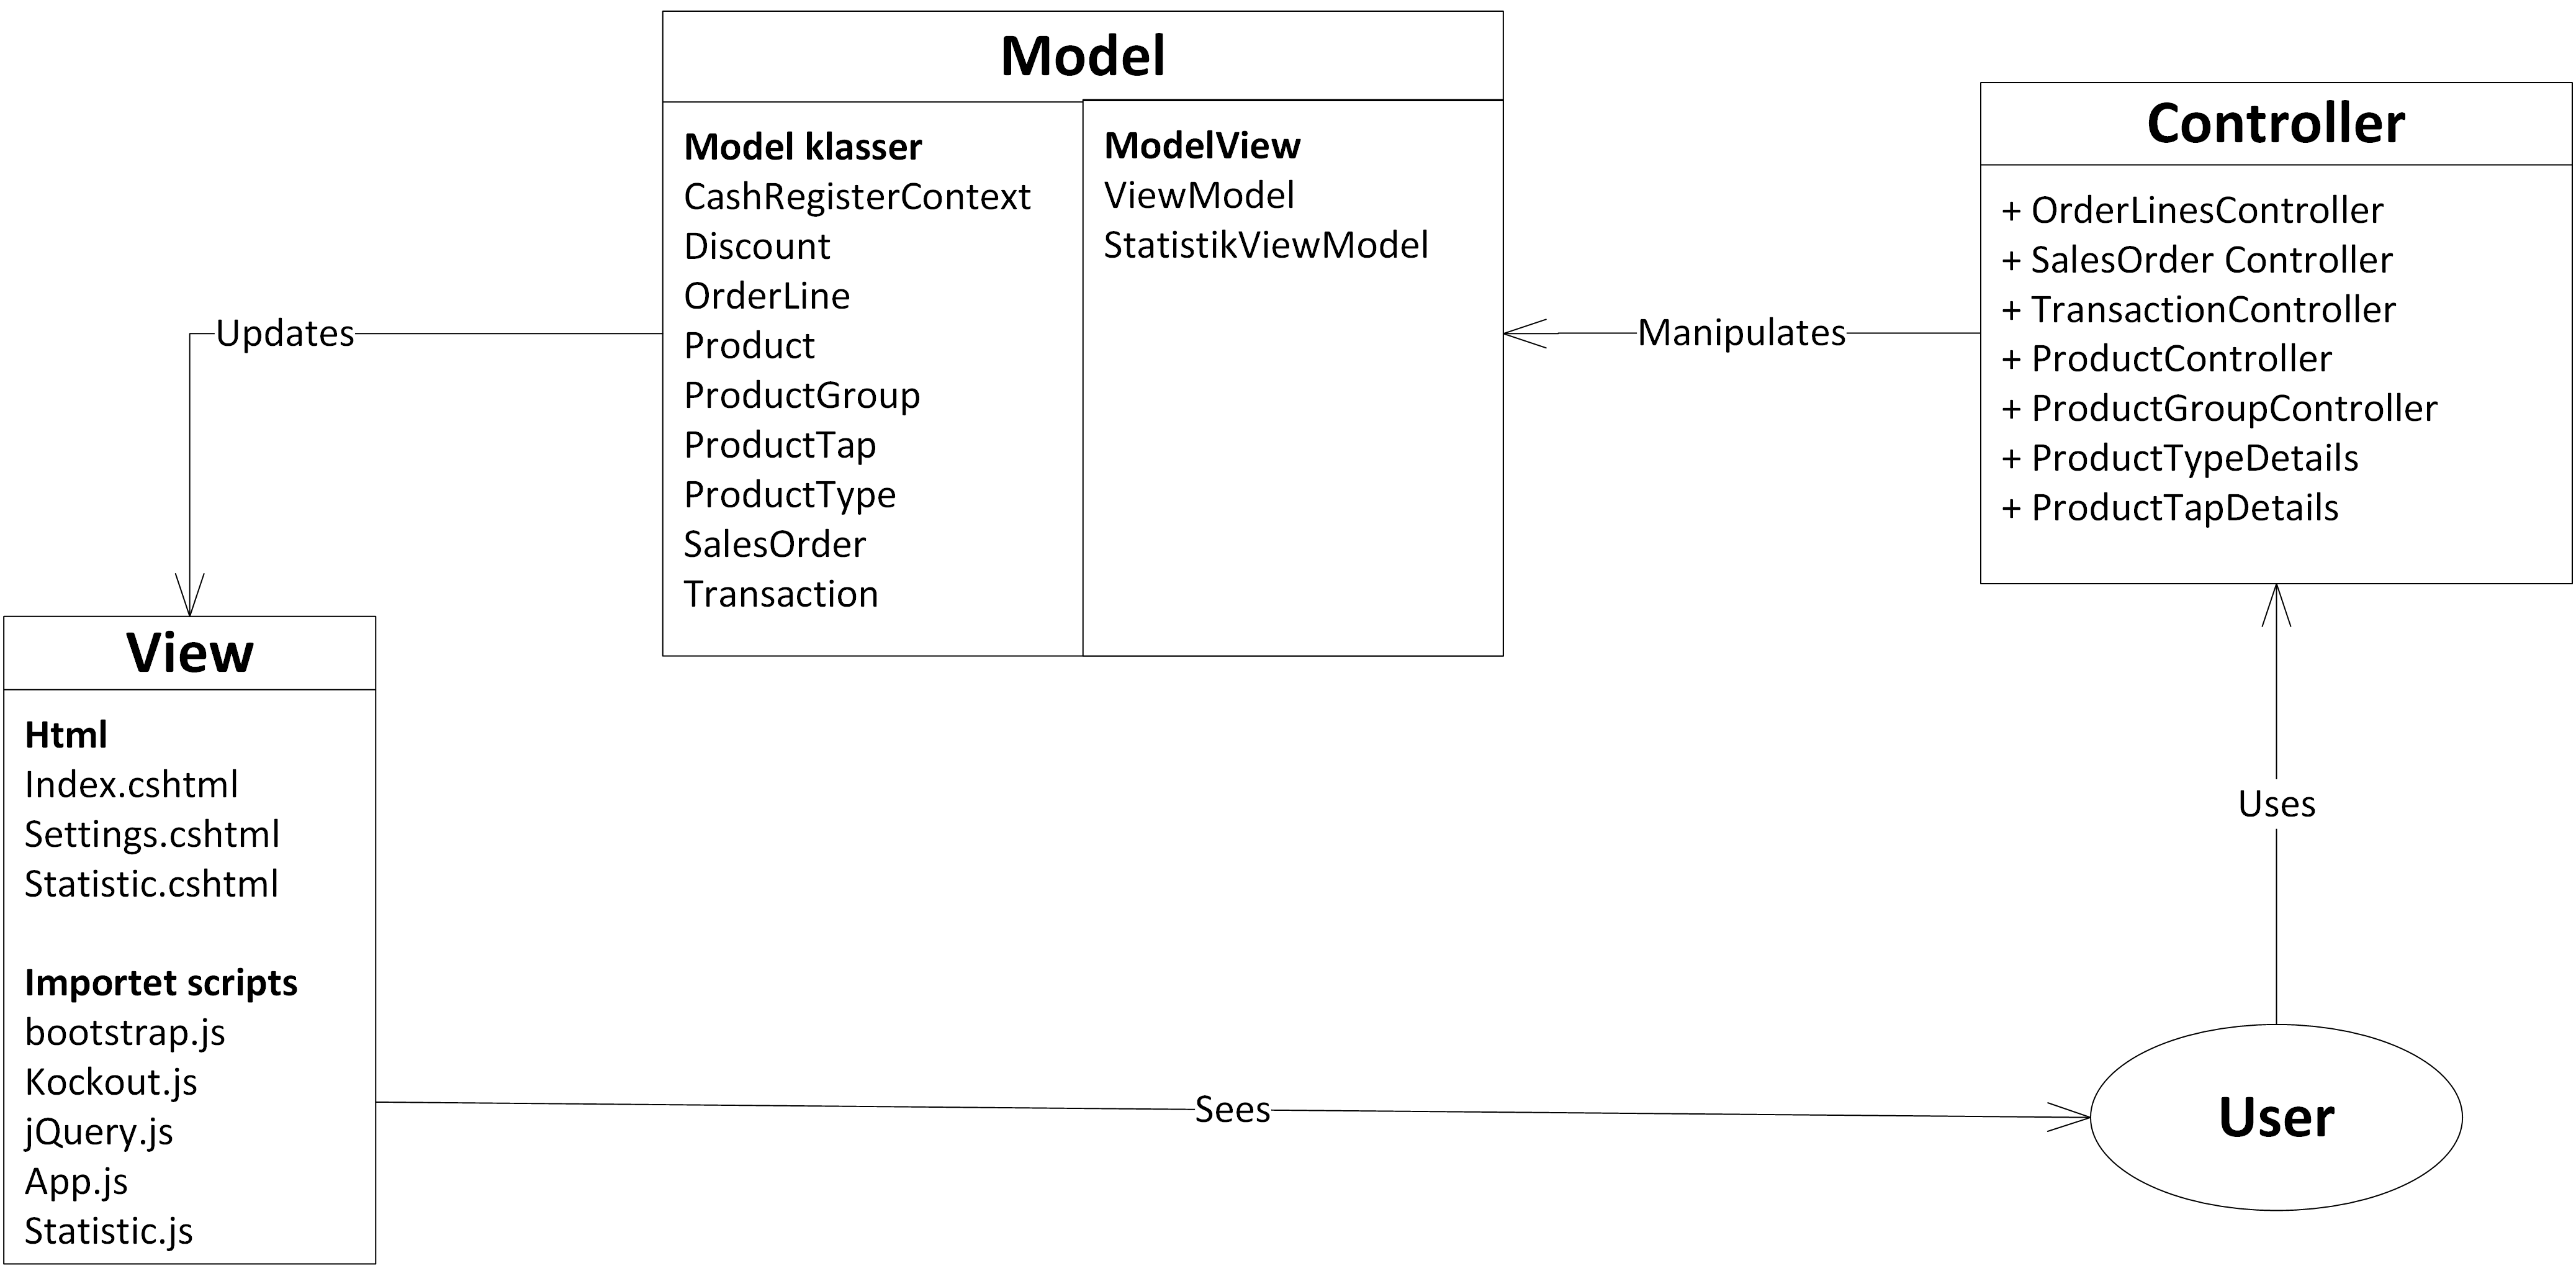
\includegraphics[width=1\textwidth]{N+1/LogicalView/WebApi/WebView/WebViewDiagram.png}
	\caption{Diagram ad WebView}
	\label{fig:Diagram_WebView}
\end{figure}

På figur \ref{fig:WebApi/WebView_SEQ} ses et sequens diagram af WebViewet. Her laver Clienten en http requst til webAPI controlleren, controlleren henter data models der har sit data fra databasen. Det data controlleren har fra models bliver sendt videre til view der formaterer et output via noget html, css og javascript kode. 
\newline
\newline
Ved ændringer af data, som f.eks. kunne være at der bliver tilføjet et objekt, så bliver der udført et asynkron http (Ajax) request, som anvender controllerens POST, til at oprette et nyt object og sætte det i databasen.  

\Diagram{0.85}{SEQ}{WebApi/WebView}{WebView}{LogicalView}